
\section*{Problema P7.35}

\renewcommand*\thesection{7.35}
\numberwithin{equation}{section}
\numberwithin{figure}{section}

\begin{center}
    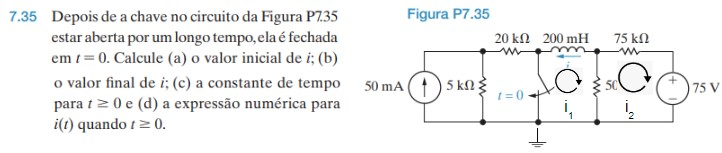
\includegraphics[scale=1.0]{P7.35.jpg}
\end{center}

\subsection*{(a)}

Para calcular o valor inicial $i(0)$ de $i$, analisamos o circuito em $t<0$, quando o indutor se comporta como um curto-circuito.
Assim, aplicando análise de malhas com as correntes $i_1$ e $i_2$. Na malha 1,

\[ 5\un{k}(i_1 - 50\un{m}) + 20\un{k}(i_1) + 50\un{k}(i_1 - i_2) = 0 \]

\[ i_1\left(5\un{k} + 20\un{k} + 50\un{k}\right) + i_2\left(- 50\un{k}\right) = ( 5\un{k})(50\un{m}) \]

\[ i_1\left(75\un{k}\right) + i_2\left(- 50\un{k}\right) = 250 \]

Para a malha 2,   

\[ 50\un{k}(i_2 - i_1) + 75\un{k}(i_2) + 75 = 0 \]

\[ i_1(-50\un{k}) + i_2(125\un{k}) = -75 \]

Com as duas equações de malha, temos o sistema linear   

\begingroup
\renewcommand*{\arraystretch}{1.5}

\[
    \begin{bmatrix}
        75\un{k} & -50\un{k}   \\
        -50\un{k}    & 125\un{k}
    \end{bmatrix}
    \begin{bmatrix}
        i_1 \\
        i_2
    \end{bmatrix}
    =
    \begin{bmatrix}
        250 \\
        75
    \end{bmatrix}
\]

\[
    \begin{bmatrix}
        75 & -50   \\
        0    & 275
    \end{bmatrix}
    \begin{bmatrix}
        i_1 \\
        i_2
    \end{bmatrix}
    =
    \begin{bmatrix}
        250\un{m} \\
        275\un{m}
    \end{bmatrix}
\]

\endgroup

\[ i_1 = 4 \un{mA} \quad , \quad i_2 = 1 \un{mA}   \]

Note que a corrente de malha $i_1$ está no sentido contrário ao definido para $i$ no enunciado. Assim, 

\[ \boxed{i(0) = - 4 \un{mA}}  \]

\subsection*{(b)}

Vamos primeiro determinar a expressão de $i(t)$ no indutor para $t>0$. Quando as chaves se fecham, temos o circuito
de \ref*{fig:7.35.1} (a). Reduzindo o circuito da Figura \ref*{fig:7.35.1} (a) via transformações de fonte, 
temos o circuito da Figura \ref*{fig:7.35.1} (b).

\begin{figure}[!htbp]
    \centering
    \caption{(a) Circuito do problema com a chave fechada. (b) Redução via transformações de fonte.}
      \centering
      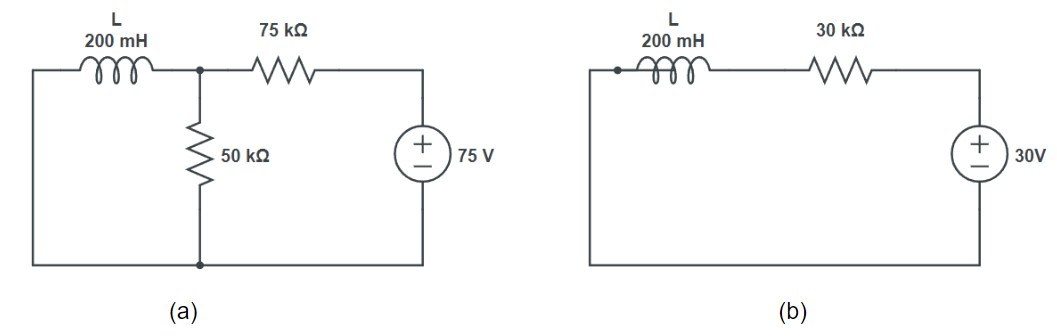
\includegraphics[scale=0.5]{P7.35-Item(b).jpg} \\
    \label{fig:7.35.1}
\end{figure}

Na Figura \ref*{fig:7.35.1} (b), aplicamos análise de malhas   

\[ L\diff{i}{t} + Ri = 30 \]

\[ \diff{i}{t} + \frac{R}{L}i = \frac{30}{L} \]

Usando o fator integrante $M(t) = e^{\frac{R}{L}t}$

\[ e^{\frac{R}{L}t}\diff{i}{t} + e^{\frac{R}{L}t}\frac{R}{L}i = e^{\frac{R}{L}t}\frac{30}{L} \]

Aplicando o inverso da regra da derivada do produto,

\[ \diff{[i \cdot e^{\frac{R}{L}t}]}{t} = e^{\frac{R}{L}t}\frac{30}{L} \]

\[ i \cdot e^{\frac{R}{L}t} = \int e^{\frac{R}{L}t}\frac{30}{L} \, dt  \]

\[ i(t)  = e^{- \frac{R}{L}t} \frac{30}{L} \frac{L}{R} \left[e^{\frac{R}{L}t} + K\right] \]

\[ i(t)  = 0.001 + Ke^{- 150000t} \]

Usando o resultado encontrado no item (a) que $i(0) = - 4 \un{mA}$, temos $K = - 0.005$. Portanto,   

\[ \boxed{i(t) = 1 - 5e^{- 150000t} \un{mA} \, , \, t \geq 0}  \]

O valor final $i(\infty)$ da corrente é    

\[ \displaystyle \lim_{t\to \infty} i(t) = 1 - 0 = 1 \un{mA}  \]

\subsection*{(c)}

A constante de tempo do circuito \ref*{fig:7.35.1} (b) é  

\[ \boxed{\tau = \frac{L}{R} = 6.67 \un{$\mu$s}}  \]

\subsection*{(d)}

Como mostrado no item (b),   

\[ \boxed{i(t) = 1 - 5e^{- 150000t} \un{mA} \, , \, t \geq 0}  \]
























